\section{Durchführung}
\label{sec:Durchführung}

\subsection{Aufbau}
\label{subsec:aufbau}

Zur Erzeugung der Mikrowellen wird ein Reflexklystron verwendet. Auf dem Hohhleiter
sind ein Isolator, ein Frequenzmesser und ein Dämpfunglied befestigt. Dies ist
in Abbildung \ref{fig:aufbau} dargestellt. Je nach
Aufgabenteil werden noch ein Stehwellendetektor, ein Abschluss, ein Kurzschluss
und ein Gleitschraubentransformator hinzugefügt. Zur Messung stehen ein Oszilloskop
und ein SWR Meter zur Verfügung.
\begin{figure}
  \centering
  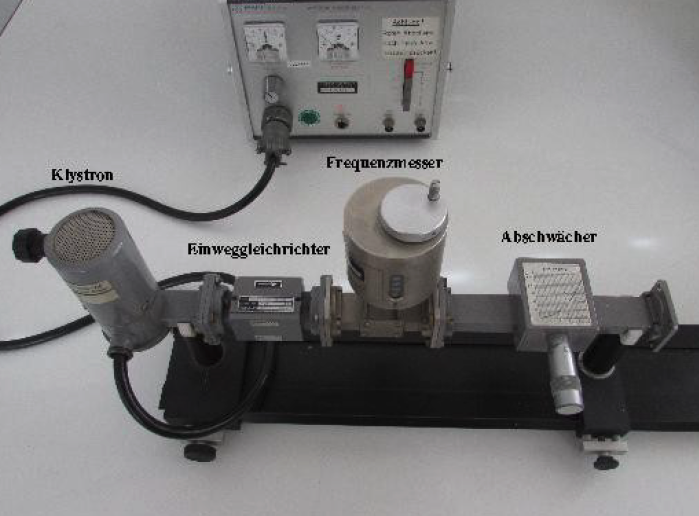
\includegraphics[width=0.7\textwidth]{data/Aufbau.png}
  \caption{Aufbau der zentralen Elemente \cite{Versuchsanleitung_neu}.}
  \label{fig:aufbau}
\end{figure}


\subsection{Untersuchung der Moden}
\label{subsec:moden}
Zur Untersuchung der Moden wird der Versuch gemäß Abbildung \ref{fig:aufbau_mode}
aufgebaut.

\begin{figure}
  \centering
  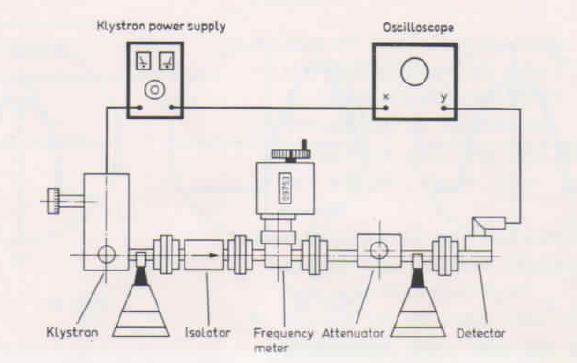
\includegraphics[width=0.7\textwidth]{data/aufbau_mode.png}
  \caption{Aufbau zum Vermessen der Moden \cite{Versuchsanleitung_alt}.}
  \label{fig:aufbau_mode}
\end{figure}

Das Dämpfungsglied wird auf \SI{32}{\decibel} eingestellt und das Signal
wird mit \SI{50}{\hertz} Sinusspannung moduliert. Das Oszilloskop
wird im xy-Modus verwendet. Dabei wird für die x-Achse der Ausgang des Netzgerätes
genutzt und auf der y-Achse die am Ende des Hohlleiters abgegriffene Spannung
verwendet. Anschließend werden Moden sichtbar gemacht. Diese haben einen
Verlauf wie er in Abbildung \ref{fig:mode} dargestellt ist.

\begin{figure}
  \centering
  \begin{subfigure}{0.3\textwidth}
    \centering
    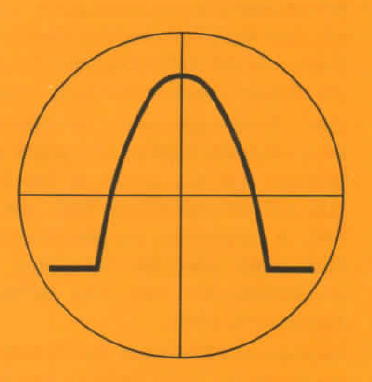
\includegraphics[height=100pt]{data/mode.png}
    \caption{Typischer Verlauf einer Mode \cite{Versuchsanleitung_alt}.}
    \label{fig:mode}
  \end{subfigure}
  \begin{subfigure}{0.3\textwidth}
    \centering
    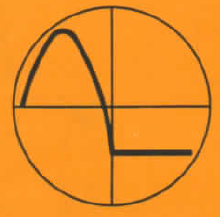
\includegraphics[height=100pt]{data/seite.png}
    \caption{Skizze zum Vermessen der Mode mithilfe von Cursorn \cite{Versuchsanleitung_alt}.}
    \label{fig:seite}
  \end{subfigure}
  \begin{subfigure}{0.3\textwidth}
    \centering
    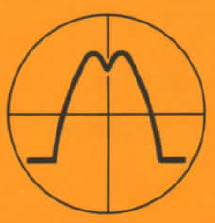
\includegraphics[height=100pt]{data/dip.png}
    \caption{Skizze zum Messen der Frequenz mithilfe des Frequenzmessers \cite{Versuchsanleitung_alt}.}
    \label{fig:dip}
  \end{subfigure}
\end{figure}

Mithilfe von Cursorn werden die Startposition des Anstiegs bzw. die Endposition
des Abfalls der Flanken (siehe Abbildung \ref{fig:seite}), sowie die Position des
Maximums und dessen Amplitude bestimmt. Die Daten für die Amplitude werden vom
Oszilloskop abgelesen. Die Werte für die Anstiege und das Maximum werden durch
Variation der Reflektorspannung mit einem Cursor als Fixpunkt bestimmt. Die Reflektorspannung,
bei der sich die Kurve so verschoben hat, dass der zu messende Punkt gerade auf dem
Cursor liegt, wird als Messwert notiert.

%\begin{figure}
%  \centering
%  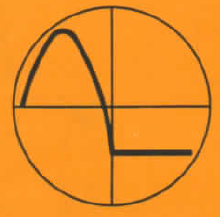
\includegraphics[width=100pt]{data/seite.png}
%  \caption{Skizze zum Vermessen der Mode mithilfe von Cursorn \cite{Versuchsanleitung_alt}.}
%  \label{fig:seite}
%\end{figure}

Mithilfe des Frequenzmessers
wird die Frequenz gemessen, indem die Frequenz so lange variiert wird, bis ein
sogenannter dip auf einem der Maxima der Moden liegt (siehe Abbildung \ref{fig:dip}).

%\begin{figure}
%  \centering
%  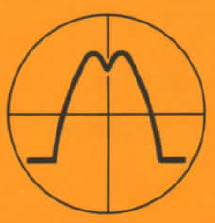
\includegraphics[width=100pt]{data/dip.png}
%  \caption{Skizze zum Messen der Frequenz mithilfe des Frequenzmessers \cite{Versuchsanleitung_alt}.}
%  \label{fig:dip}
%\end{figure}

Diese Frequenz entspricht dann der Frequenz der jeweiligen Mode.

\subsection{Bestimmung der Wellenlänge und Frequenz}
\label{subsec:frequenz}
Der Versuch wird gemäß Abbildung \ref{fig:aufbau_frequenz} Umgebaut. Das Dämpfungsglied
wird auf \SI{20}{\decibel} und die Reflektorspannung auf \SI{163}{\volt} geregelt. Zudem wird das
Signal mit einer \SI{1}{\kilo\hertz} Rechteckspannung moduliert. Anschließend wird
mithilfe des Frequenzmessers die Frequenz gemessen. Danach werden mithilfe des
Stehwellendetektors Minima gesucht und deren Positionen notiert.

\begin{figure}
  \centering
  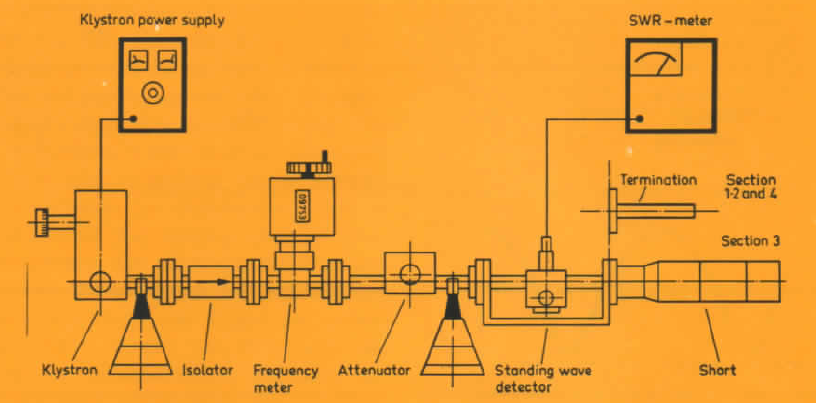
\includegraphics[width=\textwidth]{data/aufbau_frequenz.png}
  \caption{Aufbau zur Wellenlängen- und Frequenzmessung \cite{Versuchsanleitung_alt}.}
  \label{fig:aufbau_frequenz}
\end{figure}

Für einen rechteckigen Hohlleiter ergibt sich für die Frequez im freien Raum
\begin{equation}
  f=c \sqrt{\left(\frac{1}{\lambda_{\symup{g}}}\right)^2+\left(\frac{1}{2a}\right)^2} \,.
\end{equation}

\subsection{Bestimmung der Dämpfung des Mikrowellenfeldes}
\label{subsec:dämpfung}
Bei gleichem Aufbau wird die Dämpfung von 0 aus immer weiter aufgedreht. Bei jedem
vollen Dezibelschritt auf dem SWR Meter wird der Stand der Mikrometerschraube
abgelesen und das Wertepaar notiert.


\subsection{Bestimmung des Stehwellenverhältnisses}
\label{subsec:swr}

Das Stehwellenverhältnis wird über drei verschiedene Verfahren bestimmt: Die direkte
Methode, die für kleine und mittlere SWR geeignet ist, die \SI{3}{\decibel} Methode, die für hohe
SWR verwendet wird und die Abschwächer Methode, die ebenfalls für hohe SWR verwendet
wird. Es wird der Aufbau aus Abbildung \ref{fig:aufbau_swr} verwendet.

\begin{figure}
  \centering
  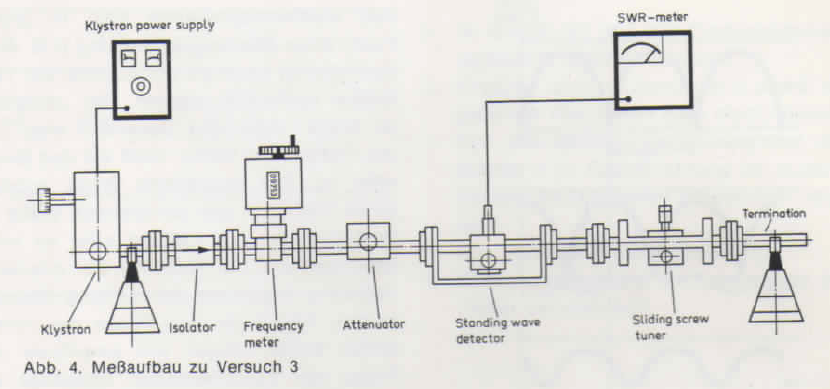
\includegraphics[width=\textwidth]{data/aufbau_swr.png}
  \caption{Aufbau zur Messung des Stehwellenverhältnisses \cite{Versuchsanleitung_alt}.}
  \label{fig:aufbau_swr}
\end{figure}

Bei der
direkten Methode wird die Sonde auf der Leitung in ein Maximum verschoben. Dieser
Wert wird dann auf dem SWR Meter mittels der Verstärkung auf 1 geregelt. Danach
wird mit der Sonde ein Minimum gesucht und der zugehörige Wert vom SWR Meter
abgelesen. Dieses Verfahren wird für Stifttiefen von 0, 3, 5, 7, und \SI{9}{\milli\meter}
durchgeführt.

Bei der \SI{3}{\decibel} Methode wird die Sonde bei \SI{9}{\milli\meter} Stifttiefe in ein
Minimum gefahren. Daraufhin wird mittels Verstärkung der Zeiger des SWR Meters auf
\SI{3}{\decibel} auf der unteren Skala geregelt. Dann werden links und rechts von dem Minimum
Stellen gesucht, an denen sich ein Vollausschlag einstellt. Die Schlittenpositionen
dieser beiden Stellen werden notiert. Es lässt sich über den Zusammenhang
\begin{equation}
  S=\sqrt{1+\frac{1}{\sin^2\left(\frac{\pi(x_1-x_2)}{\lambda_{\symup{g}}}\right)}}
  \label{eqn:3dB}
\end{equation}
das Stehwellenverhältnis bestimmen. Dabei sind $x_{\symup{i}}$ die beiden gemessenen
Schlittenpositionen.

Für die Abschwächermethode wird die Sonde bei \SI{9}{\milli\meter} Stifttiefe in ein
Minimum gefahren und das Dämpfungsglied auf \SI{20}{\decibel} eingestellt. Dann
weren gleichzeitig die Sonde verschoben und die Dämpfung erhöht, sodass sich im
Maximum die gleiche Zeigerposition wie zuvor im Minimum ergibt. Daraus kann dann
das Stehwellenverhältnis mit Hilfe von
\begin{equation}
  S=10^{\frac{A_2-A_1}{20}}
  \label{eqn:abschwaecher}
\end{equation}
berechnet werden. Hier sind $A_{\symup{i}}$ die eingestellten Dämpfungen.
